\subsection{Projektets faser (Magnus)}

Ved hjælp af logbogens afsnit og Git commit historikken er det muligt at danne et overblik af projektets faser:

\begin{table}[H]
\centering
\begin{tabular}{ll}
Testskrivning 1: & Udvalgte use cases, user stories og diagrammer \\

Testskrivning 2: & Resten af use cases, user stories og diagrammer \\

Refactoring 1: & Tests, klargøring til implementering af tests \\

\\
Implementering 1: & Core tests til hovedprogrammets klasser: App, Employee, Activity, Project  \\

Implementering 2: & Resterende tests  \\

Refactoring 2: & Ensretning af implementeret kode \\
\\ 

GUI design: & Håndtegnede figurer af GUI siderne og interaktion med programmet  \\

Implementering 3: & GUI fxml filer: knapper, labels osv. tilknyttet (tomme) controller klasser  \\

Refactoring 3: & Datohåndtering \\

Implementering 4: & GUI controllers, tilknytning til hovedprogram\\
\\

Refactoring 4: & Scope, tests \\

Slutfase: & Bug fixes, dreamlist \\


\end{tabular}
\caption{Overblik over projektets 12 faser.}
\label{tab:tidslinje}
\end{table}

\begin{figure}[H]
    \centering
    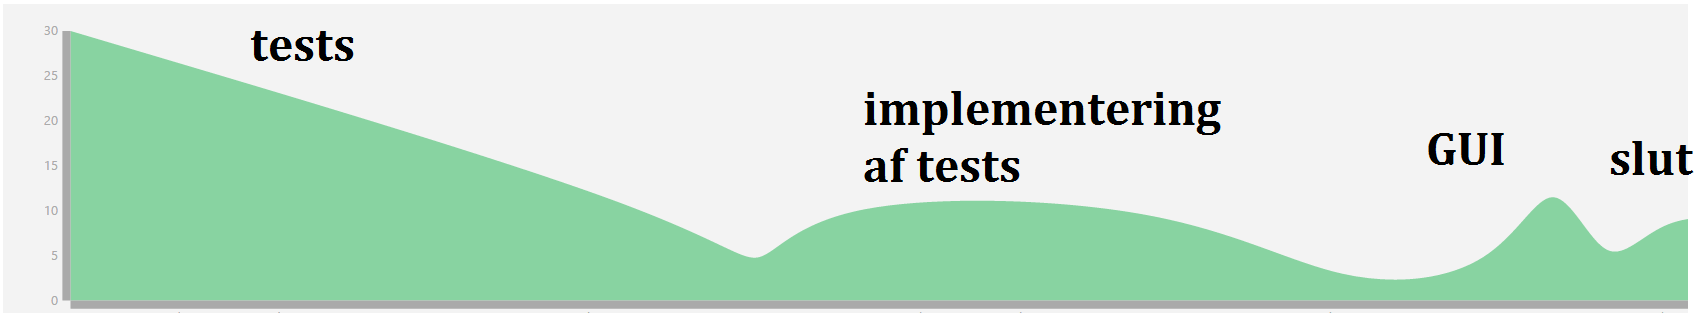
\includegraphics[width = 1.0\textwidth]{Figurer/commits_to_master.PNG}
    \caption{Gitlab oversigt over projektets gitaktivitet. De 4 peaks svarer til faserne 1-3 (tests), 4-6 (implementering af tests), 7-10 (GUI) og 11-12 (slut).}
\end{figure}

Som antydet i ovenstående liste, har gruppens arbejde været inspireret af de agile metoder præsenteret i forelæsningerne i kursus 02161. Gruppen havde også fokus på at overholde opdelingen mellem domain layer \& application layer (hovedprogrammets klasser) vs. presentation layer  (GUI’en). Hovedprogrammet fungerer uafhængigt af GUI’en, så vi kunne i princippet tilknyttet en anden GUI til programmet.

Ved indgangen til en ny fase kunne ansvaret for fx en test eller GUI controller  gives videre til et andet gruppemedlem. Eksempelvis controlleren til aktivitetssiden:

\begin{enumerate}
\item Gruppen designede kollektivt aktivitetssidens udseende og interaktion i “GUI design” fasen.
\item Magnus implementerede \texttt{activityPage.fxml} i “Implementering 3” fasen.
\item Jens tilknyttede \texttt{ActivityController.java} til hovedprogrammet i “Implementering 4” fasen.
\item Alle gruppens medlemmer har fikset bugs og foretaget logiske ændringer i \texttt{ActivityController.java} og kosmetiske  ændringer i \texttt{activityPage.fxml} i slutfasen.
\end{enumerate}
